\section{Design} \label{sec:design}

Analysis of the requirements described in \hyperref[sec:requirements]{Section \ref*{sec:requirements} } as well as those in \href{https://moodle.insttech.washington.edu/mod/resource/view.php?id=32929}{Lecture 16b} yielded the hierarchy shown in \hyperref[fig:hierarchy]{Figure \ref*{fig:hierarchy}}.
The design of each module will be discussed below.

\begin{figure}[htbp]
    \centering
    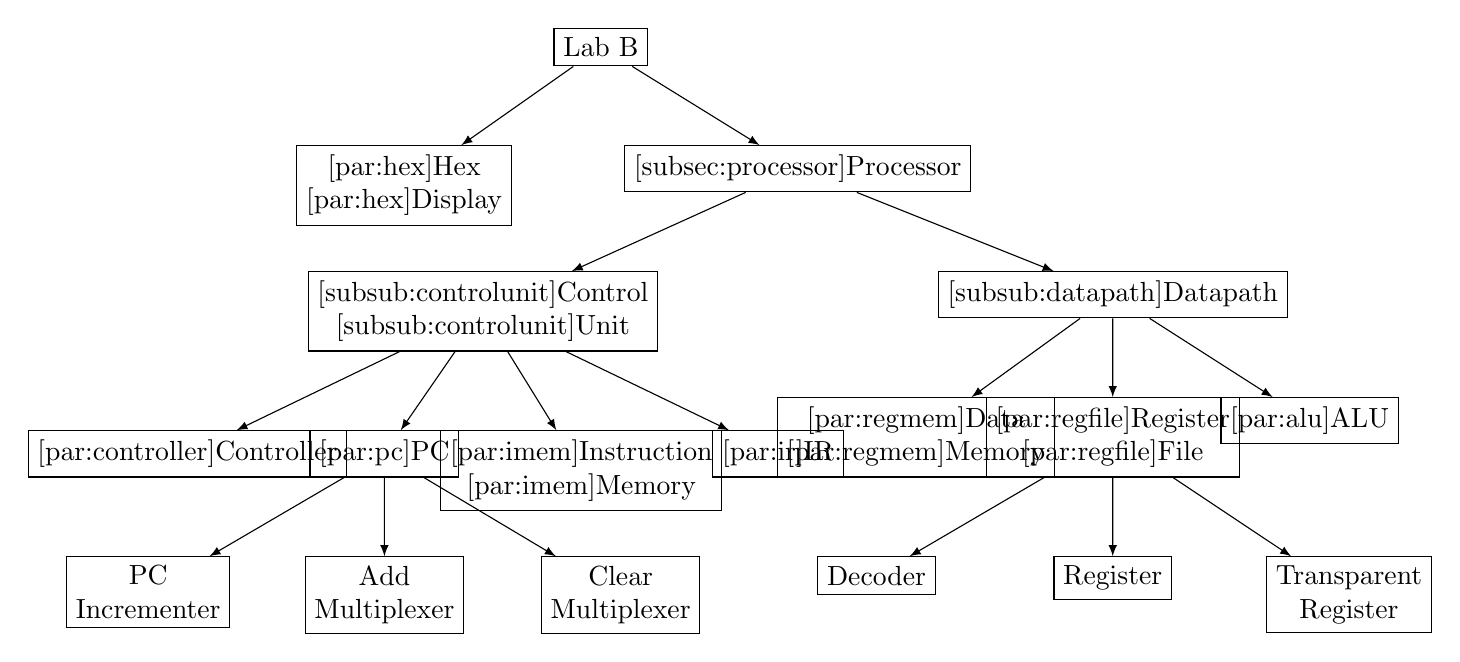
\begin{tikzpicture}[
            every node/.style={rectangle, align=center},
            level/.style={growth parent anchor=south, level distance=1cm},
            level 1/.style={sibling distance=5cm},
            level 2/.style={sibling distance=8cm},
            level 3/.style={sibling distance=2.5cm},
            level 4/.style={sibling distance=3cm},
            edge from parent/.style={draw,-latex},
            every child node/.style={anchor=north}]
        \node [draw] (top) {Lab B}
            child {node [draw] (Hex7Seg) {\hyperref[par:hex]{Hex}\\\hyperref[par:hex]{Display}}}
            child {node [draw] (Processor) {\hyperref[subsec:processor]{Processor}}
                child {node [draw] (cunit) {\hyperref[subsub:controlunit]{Control}\\\hyperref[subsub:controlunit]{Unit}}
                    child {node [draw] (controller) {\hyperref[par:controller]{Controller}}}
                    child {node [draw] (PC) {\hyperref[par:pc]{PC}}
                        child {node [draw] (PCAdderer) {PC\\Incrementer}}
                        child {node [draw] (PCUp) {Add\\Multiplexer}}
                        child {node [draw] (PCClear) {Clear\\Multiplexer}}
                    }
                    child {node [draw] (imemlpm) {\hyperref[par:imem]{Instruction}\\\hyperref[par:imem]{Memory}}}
                    child {node [draw] (IR) {\hyperref[par:ir]{IR}}}
                }
                child {node [draw] (Datapath) {\hyperref[subsub:datapath]{Datapath}}
                    child {node [draw] (RAM) {\hyperref[par:regmem]{Data}\\\hyperref[par:regmem]{Memory}}}
                    child {node [draw] (RegisterFile) {\hyperref[par:regfile]{Register}\\\hyperref[par:regfile]{File}}
                    child {node [draw] (PCClear) {Decoder}}
                        child {node [draw] (PCClear) {Register}}
                        child {node [draw] (PCClear) {Transparent\\Register}}
                    }
                    child {node [draw] (ALU) {\hyperref[par:alu]{ALU}}}
                }
            };
    \end{tikzpicture}
    \caption{Design Hierachy \label{fig:hierarchy}}
\end{figure}

The top-level module must have the properties listed below.

%TODO write up LabB.v

The file \verb|LabB.v| contains the module \verb|LabB| which satisfies these properties.
A listing can be found in the \hyperref[sec:appendix]{Appendix}, \hyperref[lst:LabB]{Listing \ref*{lst:LabB}}.

\paragraph{Hex Display} \label{par:hex}

The top-level module required a hex display Verilog module with the properties listed below.
This module was reused from Homework 2.

\begin{itemize}
    \item One four-bit input $C$.
    \item One seven-bit output $Display$.
    \item Assigns $Display$ to the appropriate value to display the character representing $C$'s value as a hexadecimal character of a seven segment display.
\end{itemize}

The file \verb|Hex7seg.v| contains the module \verb|Hex7seg| which satisfies these properties.
A listing can be found in the \hyperref[sec:appendix]{Appendix}, \hyperref[lst:hex]{Listing \ref*{lst:hex}}.

\subsection{Processor}  \label{subsec:processor}

The top-level module required a processesor Verilog modules with the properties listed below.

%TODO write up processor

The file \verb|Processor.v| contains the module \verb|Processor| which satisfies these properties.
A listing can be found in the \hyperref[sec:appendix]{Appendix}, \hyperref[lst:processor]{Listing \ref*{lst:processor}}.

\subsubsection{Control Unit} \label{subsub:controlunit}

The processor module required a control unit Verilog module with the properties listed below.

%TODO write up control unit

The file \verb|cunit.v| contains the module \verb|cunit| which satisfies these properties.
A listing can be found in the \hyperref[sec:appendix]{Appendix}, \hyperref[lst:cunit]{Listing \ref*{lst:cunit}}.

\paragraph{Program Counter} \label{par:pc}

The control unit module required a program counter Verilog module with the properties listed below.

\begin{itemize}
    \item One one-bit input $Clear$ as the active high, synchronous clear signal.
    \item One one-bit input $Up$ as the load enable signal.
    \item One one-bit input $Clock$ as the clock signal.
    \item One five-bit output $O$ as the program counter value.
\end{itemize}

The file \verb|PC.v| contains the module \verb|PC| which satisfies these properties.
A listing can be found in the \hyperref[sec:appendix]{Appendix}, \hyperref[lst:pc]{Listing \ref*{lst:pc}}.

\subparagraph{PC Incrementer}

The program counter module required a PC incrementer Verilog module with the properties listed below.

\begin{itemize}
    \item One five-bit input $I$.
    \item One five-bit output $O$ which passes the sum $I + 1$.
\end{itemize}

The file \verb|PCAdder.v| contains the module \verb|PCAdder| which satisfies these properties.
A listing can be found in the \hyperref[sec:appendix]{Appendix}, \hyperref[lst:PCAdder]{Listing \ref*{lst:PCAdder}}.

\subparagraph{Add Multiplexer}

The program counter module required an add multiplexer Verilog module with the properties listed below.

\begin{itemize}
    \item Two one-bit inputs $data0x$ and $data1x$ as the selectable inputs.
    \item One one-bit input $sel$ as the select signal.
    \item One one-bit output $result$ which passes $data0x$ or $data1x$ if $sel$ is 0 or 1 respectively.
\end{itemize}


The file \verb|PCUp.v| contains the module \verb|PCUp| which satisfies these properties from the Altera library of parameterized modules.
A listing can be found in the \hyperref[sec:appendix]{Appendix}, \hyperref[lst:PCUp]{Listing \ref*{lst:PCUp}}.

\subparagraph{Clear Multiplexer}

The program counter module required a clear multiplexer Verilog module with the properties listed below.

\begin{itemize}
    \item Two one-bit inputs $data0x$ and $data1x$ as the selectable inputs.
    \item One one-bit input $sel$ as the select signal.
    \item One one-bit output $result$ which passes $data0x$ or $data1x$ if $sel$ is 0 or 1 respectively.
\end{itemize}

The file \verb|PCClear.v| contains the module \verb|PCClear| which satisfies these properties from the Altera library of parameterized modules.
A listing can be found in the \hyperref[sec:appendix]{Appendix}, \hyperref[lst:PCClear]{Listing \ref*{lst:PCClear}}.

\paragraph{Instruction Register} \label{par:ir}

The control unit module required an instruction register Verilog module with the properties listed below.

\begin{itemize}
    \item Parameterized data bit width $N$.
    \item One one-bit input $clk$ as the clock signal.
    \item One $N$-bit input $d$ as the input value.
    \item One one-bit input $ir_\text{ld}$ as the load enable signal.
    \item One $N$-bit output $q$ as the register's value.
\end{itemize}

The file \verb|instruction_register.v| contains the module \verb|instruction_register| which satisfies these properties.
A listing can be found in the \hyperref[sec:appendix]{Appendix}, \hyperref[lst:ir]{Listing \ref*{lst:ir}}.

\paragraph{Controller} \label{par:controller}

The control unit module required controller Verilog module with the properties listed below.

\begin{itemize}
    \item One sixteen-bit input $instruction$ which accepts an intruction.
    \item One one-bit input $clk$ which acts as the clock.
    \item One one-bit output $PC_\text{clr}$ which signals to clear the program counter.
    \item One one-bit output $PC_\text{up}$ which signals to increment to program counter.
    \item One one-bit output $IR_\text{ld}$ which signals to load the instruction register.
    \item One one-bit output $RF_\text{s}$ which selects the register file.
    \item One one-bit output $RF_{W_\text{wr}}$ which signals to write enable the register file.
    \item One one-bit output $RF_{Ra_\text{rd}}$ which signals to read enable the A stream of the register file.
    \item One one-bit output $RF_{Rb_\text{rd}}$ which signals to read enable the B stream of the regoster file.
    \item One eight-bit output $D_\text{addr}$ which signals the data memory address.
    \item One one-bit output $D_wr$ which signals to write enable the data memory.
    \item One four-bit output $RF_{W_\text{addr}}$ which signals the register file's write address.
    \item One four-bit output $RF_{Ra_\text{addr}}$ which signals the register file's A stream read address.
    \item One four-bit output $RF_{Rb_\text{addr}}$ which signals the register files' B stream read address.
    \item One four-bit output $Alu_\text{s0}$ which selects the arithmetic logic unit's function.
    \item One four-bit output $State$ which signals the current state,
    \item Positive edge triggered.
    \item Quartus recognized state machine.
    \item Ten states representing each phase of each instruction.
    (See \hyperref[tab:instructions]{Table \ref*{tab:instructions}})
    \begin{itemize}
        \item \textbf{INIT}: Wait
        \item \textbf{FETCH}: Retrieve new instruction
        \item \textbf{DECODE}: Interpret instruction
        \item \textbf{NOOP}: Do nothing
        \item \textbf{LOAD\_A}: Begin load operation
        \item \textbf{LOAD\_B}: Complete load operation
        \item \textbf{STORE}: Store operation
        \item \textbf{ADD}: Addition operation
        \item \textbf{SUB}: Substraction operation
        \item \textbf{HALT}: Stop all operations
    \end{itemize}
\end{itemize}

The file \verb|controller.v| contains the module \verb|controller| which satisfies these properties.
A listing can be found in the \hyperref[sec:appendix]{Appendix}, \hyperref[lst:controller]{Listing \ref*{lst:controller}}.

\paragraph{Instruction Memory} \label{par:imem}

The control unit module required an instruction memory Verilog module with the properties listed below.

\begin{itemize}
    \item One five-bit input $address$ as the data address.
    \item One one-bit input $clock$ as the clock signal.
    \item One sixteen-bit output $q$ as the data read signal.
\end{itemize}

The file \verb|imemlpm.v| contains the module \verb|imemlpm| which satisfies these properties from the Altera library of parameterized modules.
A listing can be found in the \hyperref[sec:appendix]{Appendix}, \hyperref[lst:imemlpm]{Listing \ref*{lst:imemlpm}}.

\subsubsection{Datapath} \label{subsub:datapath}

The processor module required datapath Verilog module with the properties listed below.

\begin{itemize}
    \item One one-bit input $Clock$ as the clock signal.
    \item One one-bit input $Reset$ as an active high, synchronous reset signal.
    \item One eight-bit input $D_\text{addr}$ as the data memory address.
    \item One one-bit input $D_\text{wr}$ as the data memory write enable signal.
    \item One four-bit input $RF_{W_\text{addr}}$ as the register file write address.
    \item One one-bit input $RF_{W_\text{wr}}$ as the register file write enable signal.
    \item One four-bit input $RF_{Ra_\text{addr}}$ as the register file stream A read address.
    \item One one-bit input $RF_{Ra_\text{rd}}$ as the register file stream A read enable signal.
    \item One four-bit input $RF_{Rb_\text{addr}}$ as the register file stream B read address.
    \item One one-bit input $RF_{Rb_\text{rd}}$ as the register file stream B read enable signal.
    \item One three-bit input $Alu_{s0}$ as the ALU function select signal.
    \item Two sixteen-bit outputs $ALU_A$ and $ALU_B$ as the ALU A- and B-side inputs respectively.
    \item One sixteen-bit output $RQ0$ as the first register file entry.
    \item One sixteen-bit output $Mux_\text{out}$ as register file write data input.
    \item Positive edge triggered.
\end{itemize}

The file \verb|Datapath.v| contains the module \verb|Datapath| which satisfies these properties.
A listing can be found in the \hyperref[sec:appendix]{Appendix}, \hyperref[lst:datapath]{Listing \ref*{lst:datapath}}.

\paragraph{Data Memory} \label{par:regmem}

The datapath module required register memory Verilog module with the properties listed below.
This module was reused frome Homework 6.

\begin{itemize}
    \item One eight-bit input $address$ as the read/write address.
    \item One one-bit input $clock$ as the clock signal.
    \item One sixteen-bit input $data$ as the data to write.
    \item One one-bit input $wren$ as the write-enable signal.
    \item One sixteen-bit output $q$ as the read data stream.
    \item Positive edge-triggered.
    \item $256 \times 16$ Quartus RAM LPM with Memory Content Editor enabled.
\end{itemize}

The file \verb|ramlpm.v| contains the module \verb|ramlpm| which satisfies these properties from the Altera library of parameterized modules.
A listing can be found in the \hyperref[sec:appendix]{Appendix}, \hyperref[lst:ramlpm]{Listing \ref*{lst:ramlpm}}.

\paragraph{Register File} \label{par:regfile}

The datapath module required a register file Verilog module with the properties listed below.
This module was reused from Homework 6.

\begin{itemize}
    \item One one-bit input $Clk$ as the clock signal.
    \item One one-bit input $Reset$ as an active high reset signal.
    \item One sixteen-bit input $W_\text{data}$ as the data to write.
    \item One four-bit input $W_\text{addr}$ as the write address.
    \item One one-bit input $W_\text{en}$ as the write enable signal.
    \item Two four-bit inputs $R_\text{addr0}$ and $R_\text{addr1}$ as the A and B stream read addresses respectively.
    \item Two one-bit inputs $R_\text{en0}$ and $R_\text{en1}$ as the A and B stream read enable signals respectively.
    \item Two sixteen-bit outputs $R_\text{data0}$ and $R_\text{data1}$ as the A and B data streams respectively.
    \item One sixteen-bit output $RQ0$ which signals the contents of register 0.
    \item Positive edge triggered.
\end{itemize}

The file \verb|RegisterFile.v| contains the module \verb|RegisterFile| which satisfies these properties.
A listing can be found in the \hyperref[sec:appendix]{Appendix}, \hyperref[lst:registerfile]{Listing \ref*{lst:registerfile}}.

\subparagraph{Decoder}

The register file module required a decoder Verilog module with the properties listed below.
This module was reused from Homework 6.

\begin{itemize}
    \item Parameterized input size $N$.
    \item One $N$-bit select input $W$.
    \item One one-bit enable input $E$.
    \item One $2^N$-bit output $Y$.
    \item ``One hot'' decoder with enable.
\end{itemize}

The file \verb|DecoderN.v| contains the module \verb|DecoderN| which satisfies these properties.
A listing can be found in the \hyperref[sec:appendix]{Appendix}, \hyperref[lst:DecoderN]{Listing \ref*{lst:DecoderN}}.

\subparagraph{Register}

The register file module required a register Verilog module with the properties listed below.
This module was reused from Homework 6.

\begin{itemize}
    \item Paramerized data size $N$
    \item One one-bit input $Clk$ which acts as the clock.
    \item One one-bit input $Rst$ which acts as an active high reset.
    \item One one-bit input $Ld$ which acts as a load enable.
    \item One one-bit input $Oe0$ which acts as the A stream output enable.
    \item One one-bit input $Oe1$ which acts as the B stream output enable.
    \item One $N$-bit input $I$ which acts as the data to load.
    \item One $N$-bit output $Qz0$ which acts as the A stream switched output.
    \item One $N$-bit output $Qz1$ which acts as the B stream switched output.
    \item Positive edge triggered.
    \item Holds the value of $I$ when $Ld = 1$.
    \item Outputs the data to $Qz0$ and $Qz1$ when $Oe0$ and $Oe1$ are high respectively.
    \item Outputs high impedence otherwise.
\end{itemize}

The file \verb|RegisterOEN.v| contains the module \verb|RegisterOEN| which satisfies these properties.
A listing can be found in the \hyperref[sec:appendix]{Appendix}, \hyperref[lst:RegisterOEN]{Listing \ref*{lst:RegisterOEN}}.

\subparagraph{Transparent Register}

The register file moduule required a transparent register Verilog module witht he properties listed below.

\begin{itemize}
    \item All ports and parameters included from \verb|RegisterOEN| module.
    \item One $N$-bit output $Q_act$ which signals the register's current data.
\end{itemize}

The file \verb|RegisterOENExtraOutput.v| contains the module \verb|RegisterOENExtraOutput| which satisfies these properties.
A listing can be found in the \hyperref[sec:appendix]{Appendix}, \hyperref[lst:RegisterOENExtraOutput]{Listing \ref*{lst:RegisterOENExtraOutput}}.

\paragraph{Arithmetic Logic Unit} \label{par:alu}

The datapath module required an arithmetic logic unit Verilog module with the properties listed below.
This module was reused from Homework 6.

\begin{itemize}
    \item Two sixteen-bit inputs: $A$ and $B$.
    \item One three-bit input: $Sel$.
    \item One sixteen-bit output: $Q$.
    \item $Q$ is a function of $A$ and $B$ as selected by $Sel$ as shown in \hyperref[tab:alu]{Table \ref*{tab:alu}}..
        \begin{table}[htbp]
            \centering
            \begin{tabular}{ll}             \toprule
                $Sel$       & $Q$           \\\midrule
                0           & $0$           \\
                1           & $A + B$       \\
                2           & $A - B$       \\
                3           & $A$           \\
                4           & $A \oplus B$  \\
                5           & $A \lor B$    \\
                6           & $A \land B$   \\
                7           & $A + 1$       \\\bottomrule
            \end{tabular}
            \caption{ALU output}
            \label{tab:alu}
        \end{table}
\end{itemize}

The file \verb|ALU.v| contains the module \verb|ALU| which satisfies these properties.
A listing can be found in the \hyperref[sec:appendix]{Appendix}, \hyperref[lst:alu]{Listing \ref*{lst:alu}}.